\documentclass{beamer}
\usepackage{graphicx}
\usepackage{amsmath}
\usepackage{amsfonts}
\usepackage{amssymb}
\usepackage{tikz}
\definecolor{mygray}{rgb}{0.92,0.92,0.92}
\definecolor{FSU@Scarlet}{RGB}{140,17,17}
%\usetheme[hideothersubsections]{FSUTheme}
\usetheme{Hannover}

\begin{document}

\title{Group Meeting \\ Week 1, Spring 2019}
\author{Brandon Gusto} %
\institute{Hydro Group \\ Scientific Computing \\ Florida State University}
\date{\today}
\frame{\titlepage}

\section{Finite Volume}

\begin{frame}[shrink=15]{Finite Volume Approach}
	Here we consider the following one-dimensional refence PDE
	\begin{equation*}
		w_{t} + f(w)_{x} = s(w)
	\end{equation*}
	where $w = (\rho,\rho u,E)$ represents the primitive solution variables, and initial and boundary
	conditions are supplied. The PDE in semi-discrete form (via finite volume w/ midpoint quadrature) is
	\begin{equation*}
		(w_{j})_{t} = -\frac{1}{\triangle x} \left( f_{j+1/2} - f_{j-1/2} \right) + s_{j}
	\end{equation*}
	where the $j$ denotes spatial index. The solution is represented as cell averages
	\begin{equation*}
		w^{n}_{j} \approx \frac{1}{\triangle x} \int_{x_{j-1/2}}^{x_{j+1/2}} w(x,t_{n}) dx
	\end{equation*}
\end{frame}


\begin{frame}[shrink=15]{Finite Volume Approach}
	 The numerical flux at cell interface is a function of $2k$ local cells
	\begin{equation*}
		\hat{f}_{j+1/2} = f(w^{n}_{j-k+1},\dots,w^{n}_{j+k})
	\end{equation*}
	Computing the fluxes is usually the bulk of the computational effort (not considering overhead), requiring
	reconstructed states via ENO/WENO or TVD limiters, and Riemann solver.

\end{frame}


\section{Multiresolution}

\begin{frame}[shrink=15]{Multiresolution Representation}
	Define multiple, nested grids
	\begin{equation*}
		G^{l} = \left\{ x^{l}_{j} \right\}_{j=0}^{N_{l}}
	\end{equation*}
	where the number of cells per level $l$ is $N_{l}$ and the cell width is
	\begin{equation*}
		h_{l} = \frac{b-a}{N_{l}}
	\end{equation*}
	The aim is to decompose the field at the finest (given) level of resolution into a representation at a
	coarse level plus a series of differences at each finer level. The differences provide information about the
	function's regularity.
\end{frame}


\begin{frame}[shrink=15]{Multiresolution Representation}
	Consider some quantity of interest, $c(x)$. This will be represented as cell averages $c_{j}^{l}$ at each
	level $l$. At some level $l$ (coarse) the field at level $l-1$ (fine) is represented by a prediction from
	values at level $l$. A Lagrange interpolating polynomial is used to preserve the cell averages.
	\begin{figure}
	    \centering
	    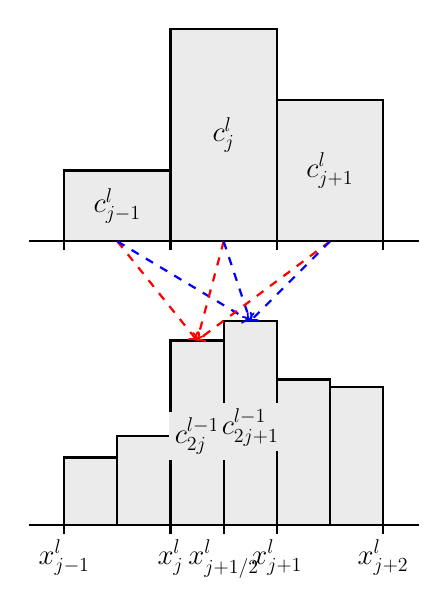
\begin{tikzpicture}[thick,scale=0.45, every node/.style={scale=0.6}]
		\draw[fill=mygray] (0,0) -- (0,2)-- (3,2) -- (3,0);
		\draw[fill=mygray] (3,0) -- (3,6) -- (6,6) -- (6,0);
		\draw[fill=mygray] (6,0) -- (6,4) -- (9,4) -- (9,0);
		\draw[fill=mygray] (-1,0) -- (10,0);
		\node at (1.5,1) {\LARGE $c^{l}_{j-1}$};
		\node at (4.5,3) {\LARGE $c^{l}_{j}$};
		\node at (7.5,2) {\LARGE $c^{l}_{j+1}$};
		\draw (0,0) -- (0,-0.25);
		\draw (3,0) -- (3,-0.25);
		\draw (6,0) -- (6,-0.25);
		\draw (9,0) -- (9,-0.25);

		% -8 is y-axis baseline for this one
		\draw[fill=mygray] (0,-8) -- (0,-6.1) -- (1.5,-6.1) -- (1.5,-8);
		\draw[fill=mygray] (1.5,-8) -- (1.5,-5.5) -- (3,-5.5) -- (3,-8);
		\draw[fill=mygray] (3,-8) -- (3,-2.8) -- (4.5,-2.8) -- (4.5,-8);
		\draw[fill=mygray] (4.5,-8) -- (4.5,-2.25) -- (6,-2.25) -- (6,-8);
		\draw[fill=mygray] (6,-8) -- (6,-3.9) -- (7.5,-3.9) -- (7.5,-8);
		\draw[fill=mygray] (7.5,-8) -- (7.5,-4.1) -- (9,-4.1) -- (9,-8);
		\draw[fill=mygray] (-1,-8) -- (10,-8);
		\node[fill=mygray] at (3.75,-5.5) {\LARGE $c^{l-1}_{2j}$};
		\node[fill=mygray] at (5.25,-5.25) {\LARGE $c^{l-1}_{2j+1}$};
		\draw (0,-8) -- (0,-8.25);
		\draw (3,-8) -- (3,-8.25);
		\draw (4.5,-8) -- (4.5,-8.25);
		\draw (6,-8) -- (6,-8.25);
		\draw (9,-8) -- (9,-8.25);

		% arrows
		\draw[red,dashed,->] (1.5,0) -- (3.75,-2.8);
		\draw[blue,dashed,->] (1.5,0) -- (5.25,-2.25);
		\draw[red,dashed,->] (4.5,0) -- (3.75,-2.8);
		\draw[blue,dashed,->] (4.5,0) -- (5.25,-2.25);
		\draw[red,dashed,->] (7.5,0) -- (3.75,-2.8);
		\draw[blue,dashed,->] (7.5,0) -- (5.25,-2.25);

		% ticj text
		\node[below] at (0,-8.25) {\LARGE $x^{l}_{j-1}$};
		\node[below] at (3,-8.25) {\LARGE $x^{l}_{j}$};
		\node[below] at (4.5,-8.25) {\LARGE $x^{l}_{j+1/2}$};
		\node[below] at (6,-8.25) {\LARGE $x^{l}_{j+1}$};
		\node[below] at (9,-8.25) {\LARGE $x^{l}_{j+2}$};

	    \end{tikzpicture}
	\end{figure}
	
\end{frame}


\begin{frame}[shrink=15]{Multiresolution Representation}
	For a third order polynomial, the prediction is
	\begin{align*}
		\hat{c}^{l-1}_{2j} = c^{l}_{j} + \frac{1}{8} \left( c^{l}_{j-1} - c^{l}_{j+1} \right) \\
		\hat{c}^{l-1}_{2j+1} = c^{l}_{j} - \frac{1}{8} \left( c^{l}_{j-1} - c^{l}_{j+1} \right)
	\end{align*}
	and the detail coefficient for the cell corresponding to $c^{l}_{j}$ is
	\begin{equation*}
		d^{l}_{j} = c_{2j+1}^{l-1} - \hat{c}_{2j+1}^{l-1}
	\end{equation*}
	The value of this coefficient is indicitive of the smoothness of the function in that vicinity. Doing this at
	each level of resolution provides the desired information.
	
\end{frame}


\section{MR Code}

\begin{frame}[shrink=15]{Multiresolution Code - Examples}
	\begin{figure}
		\center
		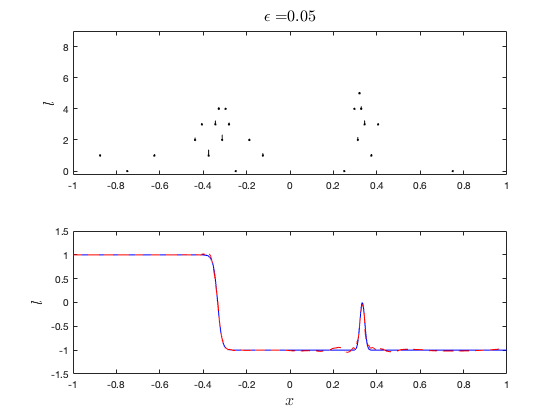
\includegraphics[scale=0.5]{plots/spike-low.png}
		\caption{Coarse approximation (large threshold value).}
	\end{figure}	
\end{frame}


\begin{frame}[shrink=15]{Multiresolution Code - Examples}
	\begin{figure}
		\center
		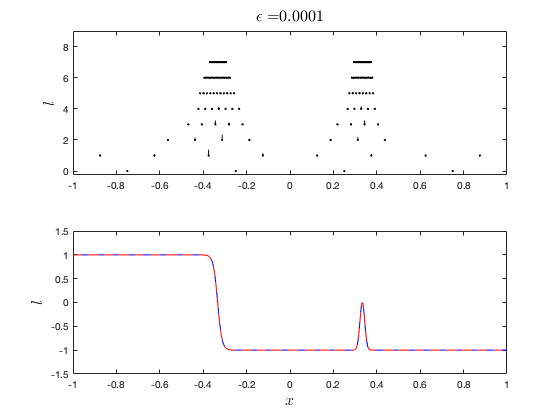
\includegraphics[scale=0.5]{plots/spike-med.png}
		\caption{Better approximation (smaller threshold value).}
	\end{figure}	
\end{frame}


\begin{frame}[shrink=15]{Multiresolution Code - Examples}
	\begin{figure}
		\center
		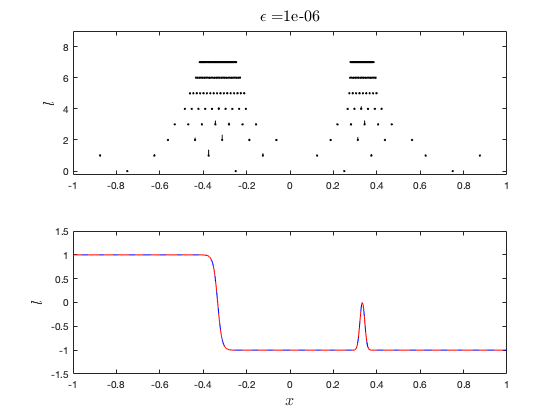
\includegraphics[scale=0.5]{plots/spike-hi.png}
		\caption{Even better approximation (even smaller threshold value).}
	\end{figure}	
\end{frame}


\begin{frame}[shrink=15]{Multiresolution Code - Examples}
	\begin{figure}
		\center
		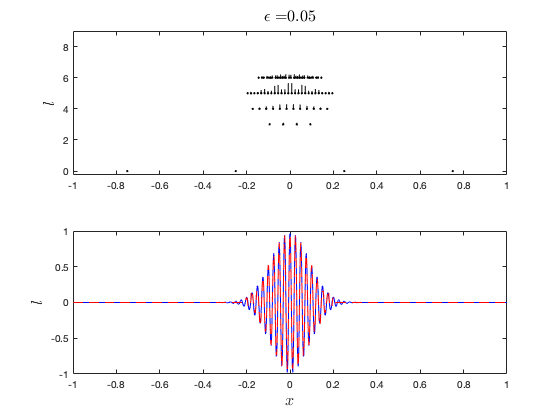
\includegraphics[scale=0.5]{plots/wiggle-low.png}
		\caption{Coarse approximation (large threshold value).}
	\end{figure}	
\end{frame}


\begin{frame}[shrink=15]{Multiresolution Code - Examples}
	\begin{figure}
		\center
		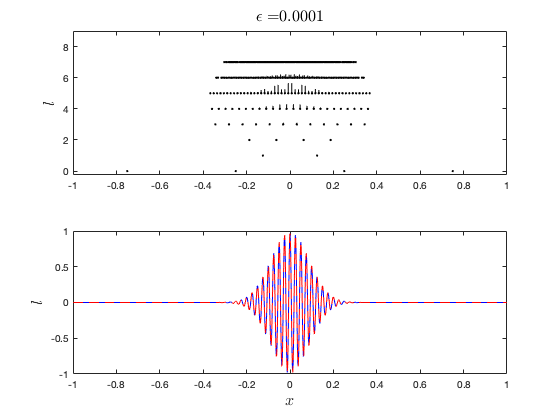
\includegraphics[scale=0.5]{plots/wiggle-med.png}
		\caption{Better approximation (smaller threshold value).}
	\end{figure}	
\end{frame}


\begin{frame}[shrink=15]{Multiresolution Code - Examples}
	\begin{figure}
		\center
		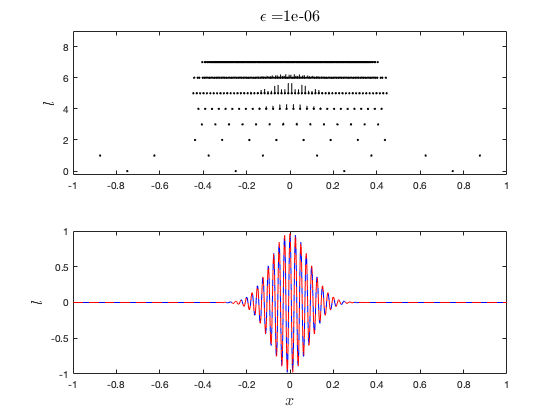
\includegraphics[scale=0.5]{plots/wiggle-hi.png}
		\caption{Even better approximation (even smaller threshold value).}
	\end{figure}	
\end{frame}


\section{Applications}
\begin{frame}[shrink=15]{Applications of Multiresolution to Finite Volume}
	What could we do with such information?
	\begin{enumerate}
		\item use regularity information to adapt the grid (just like AMR)
		\item use regularity information to reduce number of costly flux evaluations
	\end{enumerate}
	The first option is well established in the literature, and so is the second. But all production codes
	use AMR already... can we boost AMR with option 2? 
\end{frame}


\end{document}
